\subsection*{Problema 11}
\textbf{Enunciado:} Calcular la integral:
\begin{equation*}
\int \dfrac{dx}{\cos x + \sin x}
\end{equation*}

\textbf{Solución:}
Para resolver la integral dada, utilizamos la identidad trigonométrica para la combinación de seno y coseno en el denominador:
\begin{equation*}
\cos x + \sin x = \sqrt{2}\sin\left(x + \dfrac{\pi}{4}\right)
\end{equation*}

Sustituyendo esta identidad en la integral, obtenemos:
\begin{align*}
\int \dfrac{dx}{\cos x + \sin x} &= \int \dfrac{dx}{\sqrt{2}\sin\left(x + \dfrac{\pi}{4}\right)} \\
&= \dfrac{1}{\sqrt{2}} \int \csc\left(x + \dfrac{\pi}{4}\right) dx
\end{align*}

Recordamos la fórmula estándar para la integral de la cosecante:
\begin{equation*}
\int \csc(u) du = \ln\left|\csc(u) - \cot(u)\right| + C
\end{equation*}

Aplicando esta fórmula con $u = x + \dfrac{\pi}{4}$ y $du = dx$, la integral se convierte en:
\begin{align*}
&= \dfrac{1}{\sqrt{2}} \ln\left| \csc\left(x + \dfrac{\pi}{4}\right) \right. \\
&\quad \left. - \cot\left(x + \dfrac{\pi}{4}\right) \right| + C
\end{align*}

Podemos expresar el resultado en términos de funciones seno y coseno originales utilizando las definiciones trigonométricas:
\begin{align*}
\csc\left(x + \dfrac{\pi}{4}\right) &= \dfrac{\sqrt{2}}{\sin x + \cos x} \\
\cot\left(x + \dfrac{\pi}{4}\right) &= \dfrac{\cos x - \sin x}{\sin x + \cos x}
\end{align*}

Sustituyendo estas relaciones de regreso, el resultado final de la integral indefinida es:
\begin{align*}
&= \dfrac{1}{\sqrt{2}} \ln\left| \dfrac{\sqrt{2} - \cos x + \sin x}{\sin x + \cos x} \right| + C
\end{align*}

\begin{figure}[H]
	\centering
	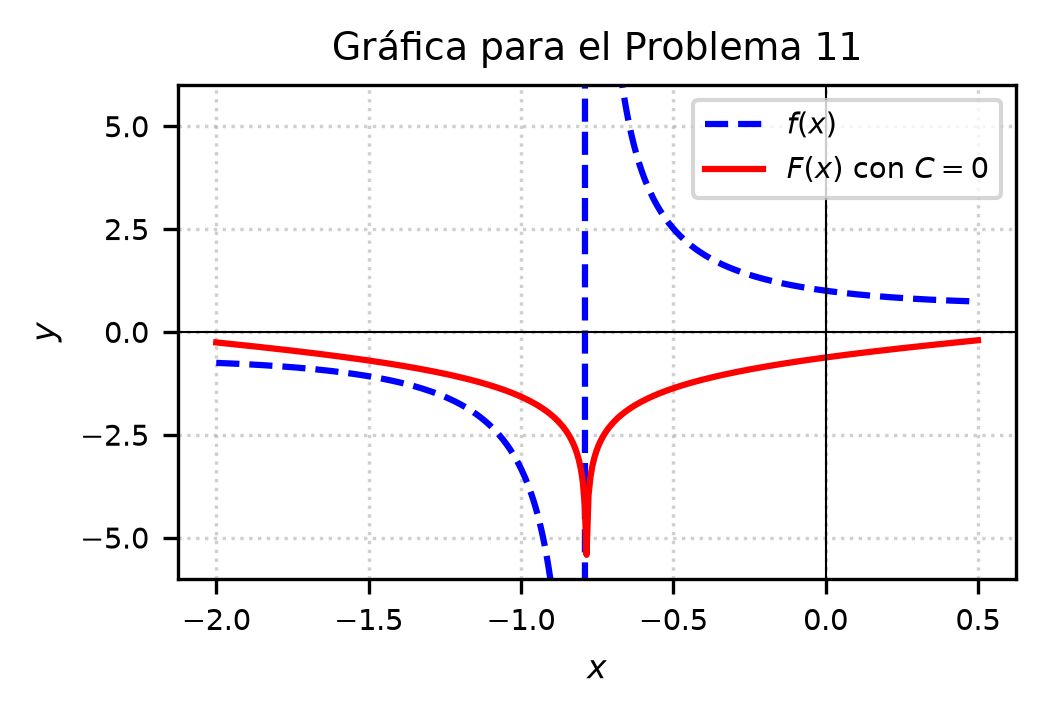
\includegraphics[width=\columnwidth]{semana_04/graficas/SEM04_P11_grafica.png}
	\caption{Representación gráfica de $f(x)$ y su antiderivada $F(x)$ evaluada para la constante de integración $C = 0$ (Problema 11).}
	\label{fig:problema11}
\end{figure}
